% compile: pdflatex  -shell-escape Erlang_Jevtic_Mrdak_Dimic_Gajic.tex
% !TEX encoding = UTF-8 Unicode

\documentclass[a4paper]{article}

\usepackage{color}
\usepackage{url}
\usepackage[T2A]{fontenc} % enable Cyrillic fonts
\usepackage[utf8]{inputenc} % make weird characters work
\usepackage{graphicx}
\usepackage{amsthm}
\newtheorem{definition}{Definicija}

\usepackage[english,serbian]{babel}

\usepackage[unicode]{hyperref}
\hypersetup{colorlinks,citecolor=green,filecolor=green,linkcolor=blue,urlcolor=blue}

\newtheorem{primer}{Primer}[section]

\usepackage{minted}
\usemintedstyle{colorful}

\usepackage{tikz}
\def\checkmark{\tikz\fill[scale=0.4](0,.35) -- (.25,0) -- (1,.7) -- (.25,.15) -- cycle;}

\usepackage{listings}
\lstset{language=erlang}

\begin{document}

\title{Erlang - funkcionalno rešenje za konkurentni svet\\ \small{Seminarski rad u okviru kursa\\Metodologija stručnog i naučnog rada\\ Matematički fakultet}}

\author{Tijana Jevtić, Jelena Mrdak, David Dimić, Zorana Gajić\\
tijanatijanajevtic@gmail.com, mrdakj@gmail.com,\\daviddimic@hotmail.com, zokaaa\_gajich@bk.ru}
\date{6.~april 2019.}
\maketitle

\abstract{
U ovom radu je prikazan programski jezik Erlang iz različitih uglova.
Kroz niz poglavlja i primera, ispričana je njegova istorija - kad, kako, gde i zašto je nastao, 
po čemu je karakterističan, šta ga to izdvaja od drugih programskih jezika, koji su to 
koncepti koji su svojevrsni Erlangu.
Nakon čitanja rada, čitalac će imati globalnu sliku o jeziku i detaljniji pogled na neke važne koncepte, 
kao i uvid u korišćenu literaturu koju može konsultovati radi daljeg informisanja o temi.

\setcounter{tocdepth}{1} 
\tableofcontents

\newpage

\section{Uvod}
\label{sec:uvod}
%TODO
uvod bla bla bla

\section{Nastanak i istorijski razvoj}
\label{sec:nastanak}

1981. godine je oformljena nova laboratorija, Erikson CSLab (eng.~{\em The Ericsson CSLab}) u okviru firme Erikson sa
ciljem da predlaže i stvara nove arhitekture, koncepte i strukture za buduće softverske sisteme.
Eksperimentisanje sa dodavanjem konkurentnih procesa u programski jezik Prolog je bio jedan
od projekata Erikson CSLab-a i predstavlja začetak novog programskog jezika.
Taj programski jezik je 1987. godine nazvan Erlang
\footnote{Erlang je jedinica saobraćaja u oblasti telekomunikacija 
i predstavlja kontinuirano korišćenje jednog kanala 
(npr. ako jedna osoba obavi jedan poziv telefonom u trajanju od sat vremena, 
tada se kaže da sistem ima 1 Erlang saobraćaja na tom kanalu).}.    
Sve do 1990., Erlang se mogao posmatrati kao dijalekt Prologa. Od tada, Erlang
ima svoju sintaksu i postoji kao potpuno samostalan programski jezik.
Godine rada su rezultirale u sve bržim, boljim i stabilnijim verzijama jezika, kao
i u nastanku standardne biblioteke OTP (eng.~{\em The Open Telecom Platform}) \cite{phdthesis}.
Od decembra 1998. godine, Erlang i OTP su postali deo slobodnog softvera (eng.~{\em open source software})
i mogu se slobodno preuzeti sa Erlangovog zvaničnog sajta \cite{sajt}.
Danas, veliki broj kompanija koristi Erlang u razvoju
svojih softverskih rešenja. Neke od njih su: Erikson, Motorola, Votsap (eng.~{\em Whatsapp}), 
Jahu (eng.~{\em Yahoo!}), Amazon, Fejsbuk (eng.~{\em Facebook}).


\subsection{Uticaji}
\label{subsec:uticaji}

Erlang je funkcionalan i konkurentan programski jezik.
Na njega, kao na funkcionalan jezik, uticao je Lisp funkcionalnom paradigmom koju je 
prvi predstavio. Na planu konkurentnosti Erlang je svojevrstan primer (detaljnije u poglavlju \ref{sec:osobine}). \\ 

Na početku, Erlang je stvaran kao neki dodatak na Prolog, vremenom prerastao u 
dijalekt Prologa, a kasnije je zbog svoje kompleksnosti i sveobuhvatnosti evoluirao
u potpuno novi programski jezik. Stoga je uticaj Prologa na Erlang bio 
neminovan. Sintaksa Erlanga u velikoj meri podseća na Prologovu 
(npr. promenljive moraju počinjati velikim slovom u oba jezika, 
svaka funkcionalna celina se završava tačkom), oba jezika u velikoj meri koriste poklapanje obrazaca
(eng.~{\em pattern matching}). \\

Sa druge strane, Erlang je uticao na nastanak programskog jezika Eliksir (eng.~{\em Elixir}). Eliksir,
uz izmenjenu Erlangovu sintaksu, dopunjenu Erlangovu standardnu biblioteku, uživa široku popularnost.

\section{Osnovna namena, svrha i mogućnosti}
\label{sec:namena}

Sa početkom od 1981. godine, jedan od zadataka Eriksonove laboratorije za računarstvo je bio pronalaženje načina za bolje programiranje aplikacija
za telekomunikacije \cite{phdthesis}. Takve aplikacije su ogromni programi i od velike važnosti je da rade sve vreme (koliko je to moguće). 
Naravno, poznato je da će tolika količina koda zasigurno imati greške, ali u toj vrsti industrije, greške mogu biti fatalne. Na primer, 
šta se dešava ako je došlo do kvara na nekoj telefonskoj liniji, a telefon nam je hitno potreban (recimo, neko ima srčani udar).
Jednostavno nije moguće zaustaviti takvu aplikaciju, popraviti je i nanovo pustiti u rad.
Kako se izboriti sa greškama u softverskim sistemima kada su one neminovne je osnovna motivacija za razvoj Erlanga \cite{phdthesis}. \\

Tako, jedna od njegovih namena jeste pisanje što sigurnijih programa koje je moguće popraviti bez potrebe za isključivanjem čitavog sistema \cite{book_joe}.
Vrlo brzi konkurentni i distribuirani programi su još jedna od Erlangovih specijalnosti. 
Poseban koncept konkurentnosti koji je implementiran u Erlangu (više u poglavlju \ref{sec:osobine}), kao i funkcionalna paradigma 
omogućavaju lako skaliranje programa i pravljenje velikih konkurentnih i distribuiranih sistema.
Velika zajednica koja se godinama razvijala je doprinela stvaranju velikog broja biblioteka i okruženja za Erlang, te proširila njegov 
inicijalni skup mogućnosti i namena \cite{book_joe}. 

\section{Osnovne osobine}
\label{sec:osobine}
Erlang je zasnovan na deklarativnoj i funckionalnoj paradigmi sa akcentom na konkurentnosti. Kao pripadnik funkcionalne paradigme poseduje sakupljač otpadaka koji upravlja memorijom u realnom vremenu tako da se ne mogu pojaviti greške programera pri rukovanju memorijom. Takođe, sistem ima ugrađenu kontrolu vremena, u smislu da se može odrediti koliko će neki proces čekati na poruku pre nego što se aktivira, pa omogućava pisanje aplikacija koje rade u mekom realnom vremenu (odziv od nekoliko milisekudni). U ovom poglavlju videćemo koji su tipovi podžani u Erlangu da bi se njegove osibine i namene opisane u poglavlju \ref{sec:namena} ostvarile, kao i neka osnovna svojstva i koncepte.



\subsection{Tipovi i promenjive}
Na raspolaganju nam je 8 primitivnih tipova. Osim uobičajnih celobrojnih, realnih vrednosti i referenci, Erlang uvodi i neke specifične tipove kao što su:

\begin{list}{•}{}
\item Atomi koji se pišu malim slovima i predstavljaju konstante i enumerisane tipove. Samo ime je njihova vrednost i nema potrebne za dodelom brojevne vrednosti
\item Binarne vrednosti omogućavaju lako i čitljivo prelamanje broja na segmente u binarni zapis na zadatoj širini. U oznaci <<vrednost:širina>>
\item Identifikatori procesa predstavljaju reference na procese. Kreiraju se funkcijom spawn
\item Portovi služe za komunikaciju sa spoljašnjim svetom. Ako su u skladu sa protokolom portova preko njih se mogu slati i primati poruke
\end{list}
 
Tu su i dve osnovne strukture: torke za fiksirani broj elemenata u njima. Definišu se sa $\{elem_1, eleme_2, ... elemt_n\}$. 
Dok su za čuvanje promenjivog broja elemenata na raspolaganju liste $[elem_1, elem_2, ...]$. Osnovni operator konstrukcije liste je $[Glava | Rep]$. U okviru listi se prikazuju i niske, za koje ne postoji ugrađeni poseban tip, već su one liste vrednost koje odgovaraju vrednostima karaktera. 
Ovo i nije neki nedostatak s obzirom na to da se niske retko koriste u telekomunikaciji.\\

Promenjive mogu biti vezane, one kojima je dodeljena neka vrednost, i slobodne. Dodela se vrši najviše jednom i vrednost vezanih promenjihiv više se ne može menjati (eng.~{\em single assignment variables}) osim ako se ne pozove funkicija f() koja sve promenjive načini slobodnim. 
Ovo je u skladu sa idejom funkcionalnih jezika da nema sporednih efekata, iako Erlang nije čisto funkcionalan jezik.


\subsection{Poklapanje obrazaca}
Svaki program sastoji se od niza funkcija pisanih poklapanjem obrazaca. Čak je i obična dodela (operatorom =) jedno poklapanje obrazaca.
Da bismo objasnili ovaj ključni koncepat potrebno je prvo da definišemo pojmove terma, obrasca i čuvara.

\theoremstyle{definition}
\begin{definition}{Osnonvni term (eng.~{\em ground term})}
se definiše kao primitivni tip, uređeni par ili lista osnovnog terma.
\end{definition}

\begin{definition}{Obrazac ili šablon (eng.~{\em pattern})}
može biti primitivni tip, promenjiva, uređeni par ili lista šablona.
Ako su u obrascu sve promenjive različite onda se on naziva primitivnim.
\end{definition}

\begin{definition}{Poklapanje obrazaca (eng.~{\em pattern matching})}
je postupak poređenja terma sa obrascem.
\end{definition}
Neformalno, ako obrazac i term imaju isti oblik, poklapanje uspeva, pri čemu će svaka promenjiva biti vezana sa podatkom na njemu odgovarajućoj poziciji. 
Ovaj proces poznat je kao {\em unifikacija}. Sledeća prva tri primera uspešno su se unifikovala, dok je u poslednjem pokušana unifikacija X sa 51 što nije uspelo kako je X već vezano za \{137, 42\}.

\begin{minted}{erlang}
Z = 2.
{X, macka} = {{137, 42}, macka}.
[Glava|Rep] = [1,2,3,4,5,6].
{X, Y} = {51, kuce}.
\end{minted}



\begin{definition}{Čuvari (eng.~{\em guards})}
su izrazi koji sadrže samo predikate oblika A op B odvojeni zarezom pri čemu su op validni binarni operatori poređenja\footnote{Operatori poređenja su: <, =<, >, =>, ==, /=, =:=, =/=}. Izraz sa čuvarima može da se evaluira samo u true ili false.
\end{definition}
Čuvari sa ključnom rečju {\em when} predstavljaju dodatno proširenje mogućnosti poklapanja obrazaca, za izvođenje jednostavnih testova i poređenja u šablonu kao u primeru funkcije za maksimum dve vrednosti:
\begin{minted}{erlang}
max(X, Y) when X > Y -> X;
max(X, Y) -> Y.
\end{minted}

\subsection{Funkcije}
%TODO
\begin{minted}{erlang}
ime_funckije(a11, a12, ... a1N) when g11, g12, ... g1N -> 
	telo1;
ime_funckije(a21, a22, ... a2N) when g21, g22, ... g2N -> 
	telo2;
...
ime_funckije(aM1, aM2, ... aMN) when gM1, gM2, ... gMN -> 
	teloM.
\end{minted}


\subsection{Podržane paradigme}
\label{subsec:paradigme}


\subsection{Koncepti}
\label{subsec:koncepti}

Jedna od osnovnih osobina Erlanga je konkurentnost i koncept na kom je zasnovana.
Reč konkurentnost se odnosi na više radnji koje se dešavaju u istom trenutku. Posmatrajući svet oko
sebe, uviđamo da je on u suštini konkurentan - u istom trenutku se dešava veliki broj procesa. \cite{phdthesis}
U tom istom trenutku, mi smo sposobni da takav svet pojmimo i odreagujemo na sve što se u njemu dešava. Dakle, mi prirodno razumemo konkurentnost.
Tako se i prirodno nameće potreba za programskim jezikom koji bi omogućavao jednostavno modelovanje sveta kakav on stvarno jeste. \\

Koncept konkurentnosti implementiran u Erlangu se zove konkurentnost slanjem poruka (eng.~{\em message passing concurrency})
i podrazumeva postojanje velikog broja procesa koji nikad ne dele memoriju, već komuniciraju isključivo asinhronim slanjem poruka \cite{book_joe}.
Sva izračunavanja se obavljaju u okviru procesa i trebalo bi da sistem bude dizajniran tako da jedan proces radi jedan mali posao.
Važno je napomenuti da procesi u Erlangu nisu procesi operativnog sistema, već Erlanga.
To je moguće zbog toga što se programi napisani u Erlangu izvršavaju na BEAM virtuelnoj mašini.
Tako, procesi u Erlangu se prave i uništavaju jako brzo, zauzimaju samo onoliko memorije koliko je neophodno, u većini slučajeva jako malo
i ponašaju se isto na svim operativnim sistemima \cite{book_joe}.
\\

Poređenja radi, koncept konkurentnosti korišćen od strane većine programskih jezika je takozvani 
koncept konkurentnosti deljenih stanja (eng.~{\em shared state concurrency}) gde procesi 
menjaju memoriju (nasuprot tome, u Erlangu vrednost promenljivoj može biti dodeljena samo jednom) \cite{book_joe}. 
U slučaju da više procesa žele da menjaju istu memoriju, tzv. kritična sekcija, potrebno je 
nekako zaštiti taj deo memorije (muteksi, katanci i dr.). U slučaju da do greške dođe baš u kritičnoj sekciji,
ostali procesi ne znaju kako da se nose sa datom situacijom i u najboljem slučaju sistem prekida sa radom. 

\begin{figure}[h!]
\begin{center}
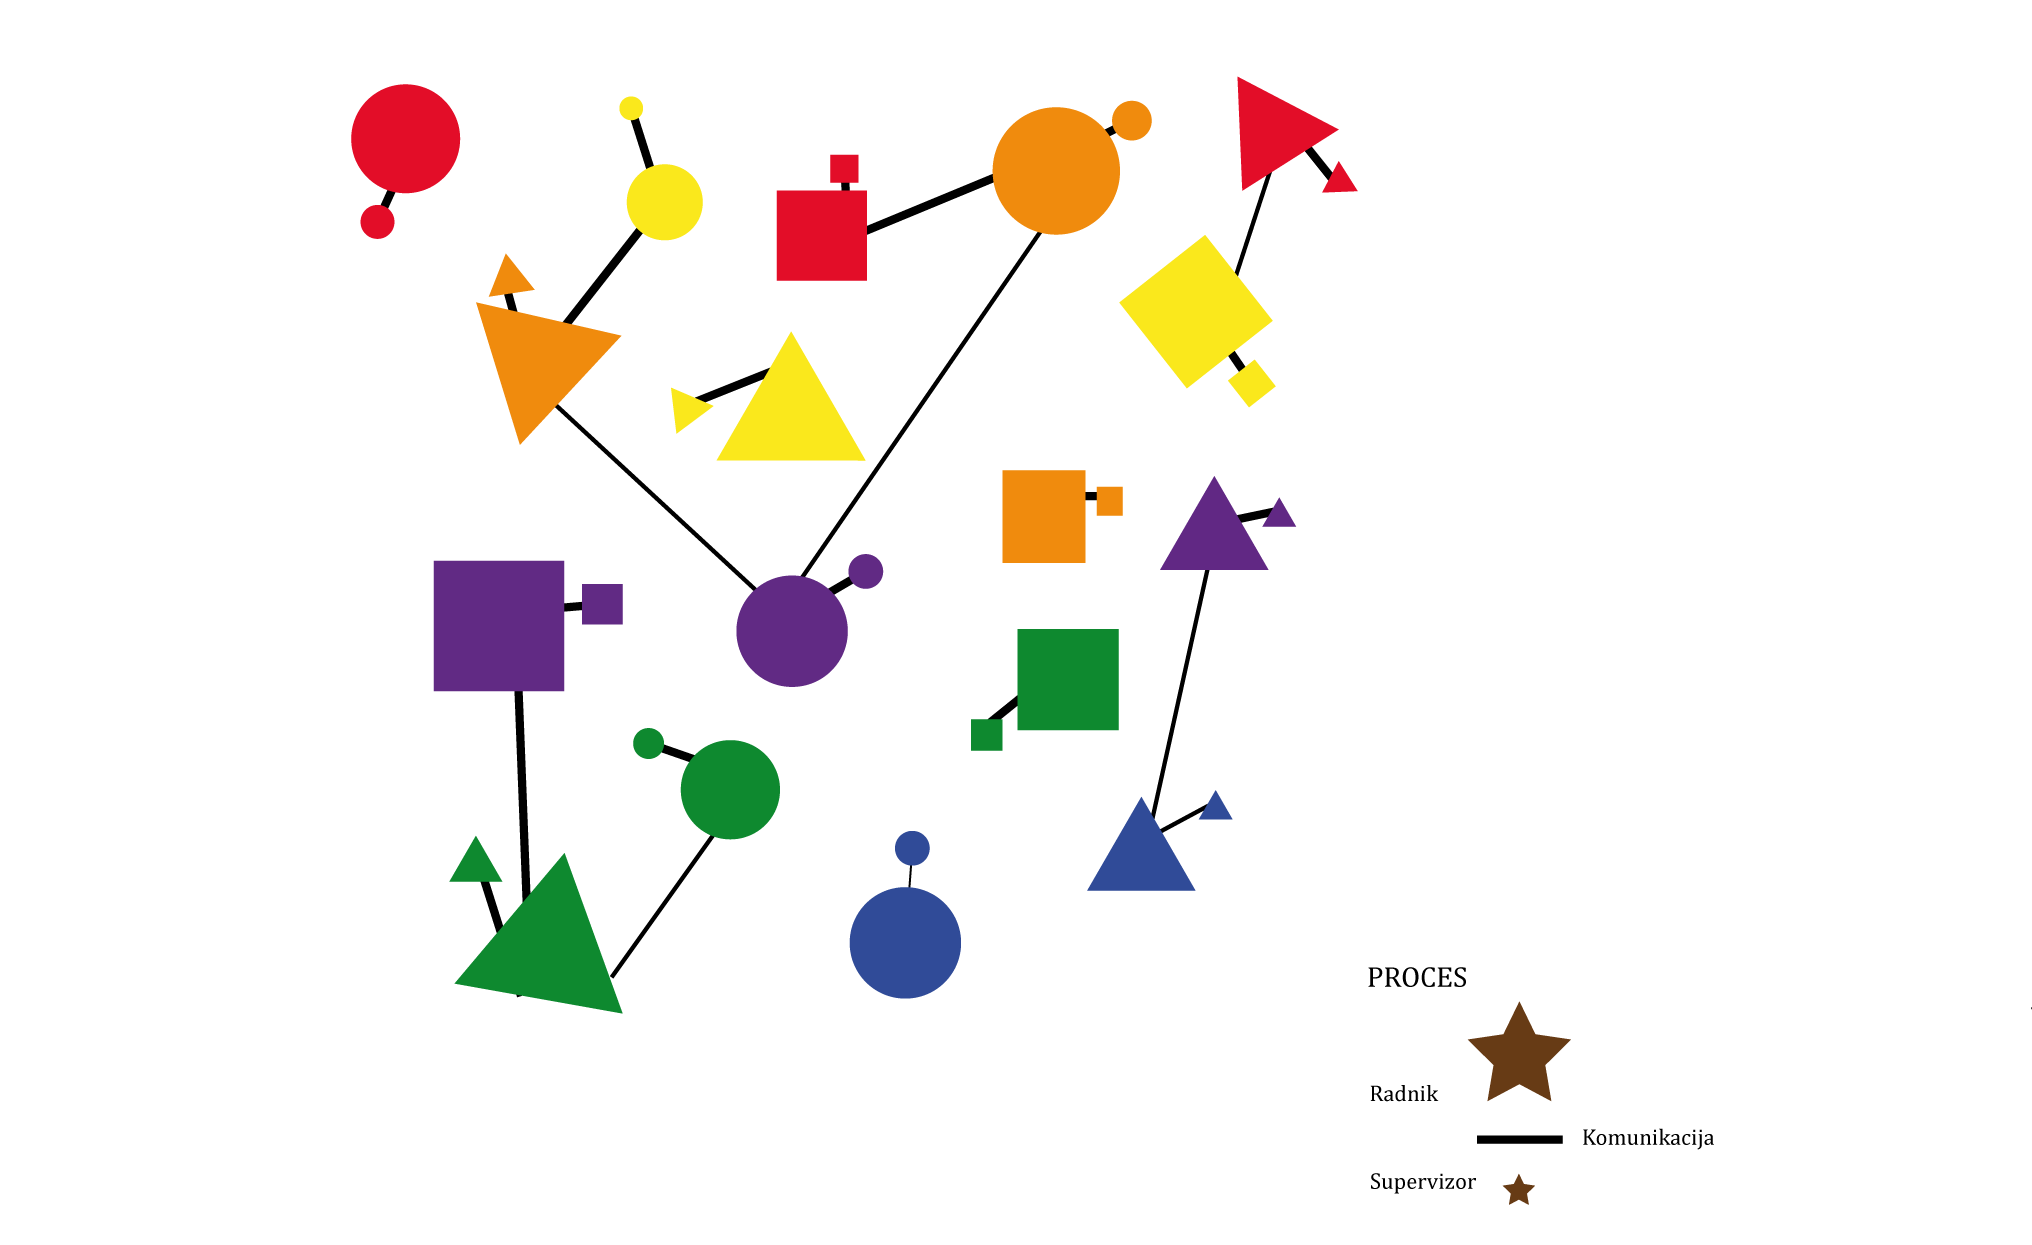
\includegraphics[scale=0.5]{actor_model.png}
\end{center}
\caption{Konkurentnost u Erlangu}
\label{fig:actor_model}
\end{figure}

\section{Okruženja (framework) i njihove karakteristike}
\label{sec:okruzenja}
Programski jezik Erlang je poznat za podržavanje skalabilnih sistema otpornih na greške (eng.~{\em scalable fault-tolerant systems}) ali takođe nudi mnoštvo mogućnosti koje ga čine odgovarajućim jezikom za veb programiranje. Naprimer mogućnost reagovanja na više korisničkih zahteva istovremeno ne razmišljajući o problemima konkurentnosti.\\

Poredili smo 3 glavna veb okruženja: {\em ChicagoBoss}, {\em Nitrogen} i {\em Zotonic}. U tabeli \ref{tab:tabela_okruzenja} smo prikazali neke interesantne osobine.\\

\begin{table}[h!]
\begin{center}
\caption{Poređenje Erlang veb okruženja}
\begin{tabular}{|c|c|c|c|}\hline
 &ChicagoBoss &Nitrogen &Zotonic \\ \hline
Razvoj zasnovan na događajima &\checkmark  &\checkmark & \checkmark  \\ \hline
Okruženje za testove &\checkmark  &\checkmark & \checkmark  \\ \hline
Generisanje koda &\checkmark & N/A & - \\ \hline
Django šabloni &\checkmark & - &\checkmark  \\ \hline
Integrisani mejl server &\checkmark & N/A &\checkmark  \\ \hline
UTF-8 u Erlang kodu &\checkmark & - &\checkmark  \\ \hline
Višejezični podaci & - & - &\checkmark  \\ \hline
Generisanje {\em JavaScript} koda & - &\checkmark & \checkmark  \\ \hline
Generisanje {\em JSON} formata &\checkmark  &\checkmark & \checkmark  \\ \hline
Integrisani WebSocket &\checkmark  &\checkmark & \checkmark  \\ \hline
 \end{tabular}
\label{tab:tabela_okruzenja}
\end{center}
\end{table} 

Okruženje {\em ChicagoBoss} sadrži sloj apstrakcije baze podataka (eng.~{\em database abstraction layer}) pod nazivom {\em BossDB} \cite{ChicagoBossDocumentation} koji je zaslužan za postavljanje upita nad bazom podataka i njeno ažuriranje. Podržani su {\em MySQL, Mnesia, Tokyo Tyrant i PostgreSQL}. Za razliku od {\em ChicagoBoss-a} {\em Nitrogen} okruženje ne podržava model podataka uopšte, a {\em Zotonic} \cite{ZotonicDocumentation} podržava isključivo {\em PostgreSQL}.\\

Takođe je interesantno videti da neka okruženja imaju integrisani mejl server koji nudi funkcije za primanje i slanje e-pošte i ostale mogućnosti, olakšavajući rad korisnicima. Naprimer slanje pošte izgleda ovako: \\

\begin{minted}{erlang}
boss_mail:send(FromAddress, ToAddress, Subject, Body)
\end{minted} 

U tabeli \ref{tab:tabela_okruzenja} smo videli da sva tri okruženja podržavaju i okruženje za testove, gde su testovi struktuirani kao stabla nastavaka (eng.~{\em trees of continuations}). Detaljnije o ovome možete pogledati u radu autora {\em ChicagoBoss} okruženja \cite{EvanMillerTesting}. Postoje gotove funkcije koje olakšavaju testiranje nekih opšte poznatih akcija kao što je provera da li je e-pošta ispravno primljena/poslata, da li je stranica na veb-u modifikovana itd. \\

{\em Django} šabloni (eng.~{\em Django templates}) \cite{DjangoTempDoc} služe za jednostavnije i brže generisanje dinamičkih HTML stranica pomoću gotovih šablona. {\em Nitrogen} ima svoje {\em Nitrogen HTML} šablone ali je u procesu prelazak na {\em Django} šablone. \\

Za {\em Nitrogen} \cite{NitrogenDocumentation} je karakteran {\em veb DSL} \cite{WebDSL} sa korišćenjem Nitrogen elemenata \cite{NitrogenDocumentation} što u suštini omogućava pisanje HTML/Javascript korišćenjem Erlang uslova pre nego HTML uslova. \\

U tabeli \ref{tab:tabela_okruzenja_serveri} možemo videti za koje servere postoji podrška u datim veb okruženjima.
\begin{table}[h!]
\begin{center}
\caption{Poređenje Erlang veb okruženja prema serverima}
\begin{tabular}{|c|c|c|c|}\hline
Server &ChicagoBoss &Nitrogen &Zotonic \\ \hline
Mochiweb &\checkmark &\checkmark &\checkmark  v(0.x) \\ \hline
Cowboy &\checkmark &\checkmark &\checkmark  v(1.0) \\ \hline
Yaws & - &\checkmark & - \\ \hline
Misultin &\checkmark & - & - \\ \hline
 \end{tabular}
\label{tab:tabela_okruzenja_serveri}
\end{center}
\end{table} 

Svaki od opisanih okruženja ima svoje prednosti i mane i zato nije jednostavno presuditi koji od ovih okruženja treba koristiti zasigurno, a koji ne treba. U zavisnosti od onoga šta je prioritet biramo odgovarajuće okruženje.

\section{Instalacija i pokretanje}
\label{sec:instalacija}

Postoji više načina da se instalira Erlang sa neophodnim paketima.
U ovom odeljku će biti predstavljena instalacija korišćenjem prekompajliranih binarnih fajlova 
za neke operativne sisteme zasnovane na Linuksovom kernelu i pokretanje na jednom od njih, kao 
i instalacija za Windows.

\subsection{Linux}
\label{subsec:instalacijaLinux}

Na operativnim sistemima zasnovanim na {\em Ubuntu}, Erlang se može instalirati sa:
{\em sudo apt-get install erlang}. \\

Nakon uspešne instalacije, Erlang kod je moguće kompajlovati
ili interpretirati i pokretati u interpretatoru.
Interpretator se pokreće kucanjem komande {\em erl} u terminalu, a iz istog
se izlazi sa {\em Ctrl+G} iza kog sledi {\em q} \cite{book_joe}.
Erlang interpretator ima u sebi ugrađen editor teksta koji je baziran na {\em emacs-u} \cite{book_fred}.
Kod iz datoteke se kompajluje komandom {\em erlc} i navođenjem imena fajla sa ekstenzijom {\em erl}.
Nakon toga se dobija izvršna datoteka sa ekstenzijom {\em beam} koja se može
pokrenuti uz navođenje adekvatnih flegova. 

\subsection{Windows}
\label{subsec:instalacijaWindows}


\section{Primeri kodova sa objašnjenjima}
\label{sec:primeri}
Po\v ce\' cemo od primera "Hello World".  
\begin{minted}{erlang}
% hello world program
-module(helloworld). 
-export([start/0]). 

start() -> 
   io:fwrite("Hello, world!\n").
\end{minted}
\begin{minted}{erlang}
> Hello, world!
\end{minted}

Nekoliko napomena:
\begin{itemize}
  \item Znak \% ozna\v cava linijski komentar.
  \item Modul je ekvivalent namespace-u u drugim jezicima.
  \item Export funkcija se koristi da bi funkcija definisana u programu mogla da se koristi. Mi defini\v semo funkciju start, a da bismo mogli da je koristimo potreban nam je export. /0 ozna\v cava da funkcija \textit{start} prima 0 argumenata.
  \item Da bismo \v zeljeni tekst prikazali u konzoli, koristimo \textbf{io} modul koji sadr\v zi potrebne IO funkcije u Erlangu.
\end{itemize}

Po\v sto smo videli kako string mo\v zemo ispisati na standardni izlaz, sada \' cemo videti kako broj mo\v zemo ispisati. Slede\' ci program prikazuje zbir dva intiger-a.

\begin{minted}{erlang}
-module(helloworld).
-export([start/0]).

start() ->
   io:fwrite("~w",[1+1]).
\end{minted}
\begin{minted}{erlang}
> 2
\end{minted}

Na sli\v can na\v cin mo\v zemo ispisivati i razne druge tipove.\\

Kao i ve\' cina funkcionalnih jezika, i Erlang podr\v zava shvatanje listi (eng. list comprehensions), \v sto ilustrujemo narednim primerima.
\begin{minted}{erlang}
> [X || X <- [1,2,a,3,4,b,5,6], X > 3].
\end{minted}
\begin{minted}{erlang}
[a,4,b,5,6]
\end{minted}
Notacija {\mintinline{erlang}{X <- [1, 2, a, ...]}} je generator, dok je izraz {\mintinline{erlang}{X>3}} filter.\\

Mo\v zemo primeniti vi\v se filtera.
\begin{minted}{erlang}
> [X || X <- [1,2,a,3,4,b,5,6], integer(X), X > 3].
\end{minted}
\begin{minted}{erlang}
[4,5,6]
\end{minted}

Tako\dj e, mogu\' ce je kombinovati i generatore. Na primer, Dekartov proizvod dve liste mo\v zemo napisati kao
\begin{minted}{erlang}
> [{X, Y} || X <- [1,2,3], Y <- [a,b]].
\end{minted}
\begin{minted}{erlang}
[{1,a},{1,b},{2,a},{2,b},{3,a},{3,b}]
\end{minted}

Algoritam QuickSort u Erlangu se mo\v ze implementirati na slede\' ci na\v cin:
\begin{minted}{erlang}
sort([Pivot|T]) ->
    sort([ X || X <- T, X < Pivot]) ++
    [Pivot] ++
    sort([ X || X <- T, X >= Pivot]);
sort([]) -> [].
\end{minted}
Izraz {\mintinline{erlang}{[X || X <- T, X < Pivot]}} e lista svih elemenata iz T koji su manji od pivota. Sli\v cno, {\mintinline{erlang}{[X || X <- T, X >= Pivot]}} je lista svih elemenata iz T koji su ve\' ci ili jednaki od pivota.\\

Neizostavna funkcija svih funkcionalnih programskih jezika jeste map.
map(F, List) je funkcija koja prima funkciju F i listu L i vra\' ca novu listu dobijenu primernom funkcije F na svaki element liste L.
\begin{minted}{erlang}
map(F, [H|T]) -> [F(H)|map(F, T)];
map(F, [])    -> [].
\end{minted}

\begin{minted}{erlang}
double(L)  -> map(fun(X) -> 2*X end, L).
\end{minted}

\begin{minted}{erlang}
> double([1,2,3,4]).
\end{minted}
\begin{minted}{erlang}
[2,4,6,8]
\end{minted}

\section{Specifičnosti}
\label{sec:specificnosti}


\section{Zaključak}
\label{sec:zakljucak}



\addcontentsline{toc}{section}{Literatura}
\appendix
\bibliography{seminarski} 
\bibliographystyle{plain}

\appendix
\section{Dodatak}



\end{document}
